% OSAC on Sheldon: sequence diagrams with boundaries. Build: pdflatex sequence-diagrams.tex (twice).
\documentclass[10pt]{article}
\usepackage[paperwidth=420mm,paperheight=297mm,margin=10mm]{geometry}
\usepackage{tikz}
\usetikzlibrary{calc,arrows.meta,positioning,fit,backgrounds,shapes.misc}
\usepackage{xcolor}
\usepackage[hidelinks]{hyperref}
\pagestyle{empty}
\definecolor{bOut}{HTML}{E3F2FD}   % outside / customer
\definecolor{bHub}{HTML}{FFF3E0}   % hub / management domain
\definecolor{bFab}{HTML}{E8F5E9}   % provider fabric manager
\definecolor{bTen}{HTML}{F3E5F5}   % tenant space (fabric + DPU + server + storage)
\definecolor{bLife}{HTML}{FFEBEE}  % lifecycle network (creation time only)
\definecolor{cHand}{HTML}{B71C1C}

% ---- sequence-diagram macros -------------------------------------------------
% \lane{id}{x}{label}            participant header at (x,0) + lifeline to depth \sdH
% \msg{y}{from}{to}{text}        solid arrow at depth y
% \rmsg{y}{from}{to}{text}       dashed (reply/response) arrow
% \self{y}{id}{text}             self-message
% \bound{x1}{x2}{title}{color}   vertical boundary (shaded column group) with a title
% \phase{y1}{y2}{title}{color}   horizontal band (time phase) with a title at the left
% \note{y}{x1}{x2}{text}         note box between depths
\newlength{\sdH}
\newcommand{\lane}[3]{%
  \node[draw,fill=white,rounded corners=2pt,align=center,minimum height=9mm,font=\footnotesize\bfseries,inner sep=3pt] (#1) at (#2,0) {#3};
  \draw[densely dashed,gray] (#1.south) -- ++(0,-\sdH);}
\newcommand{\msg}[4]{\draw[-{Stealth[length=2mm]},thick] ($(#2)+(0,-#1)$) -- ($(#3)+(0,-#1)$) node[midway,above,font=\scriptsize,align=center,fill=white,fill opacity=.85,text opacity=1,inner sep=1pt]{\stepno#4};}
\newcommand{\rmsg}[4]{\draw[-{Stealth[length=2mm]},thick,dashed] ($(#2)+(0,-#1)$) -- ($(#3)+(0,-#1)$) node[midway,above,font=\scriptsize,align=center,fill=white,fill opacity=.85,text opacity=1,inner sep=1pt]{\stepno#4};}
\newcommand{\self}[3]{\draw[-{Stealth[length=2mm]},thick] ($(#2)+(0,-#1)$) -- ++(1.1,0) -- ++(0,-0.45) -- ++(-1.1,0) node[pos=.25,right=.55,above,font=\scriptsize,align=left,anchor=south west,inner sep=1pt]{\stepno#3};}
\newcommand{\bound}[4]{\begin{pgfonlayer}{background}\fill[#4,rounded corners=4pt] (#1,0.85) rectangle (#2,-\sdH-0.3);\node[anchor=north west,font=\scriptsize\bfseries,text=black!60] at (#1+0.1,0.85) {#3};\end{pgfonlayer}}
\newcommand{\phase}[4]{\begin{pgfonlayer}{background}\fill[#4,opacity=.35] (-1.2,-#1) rectangle (\sdW,-#2);\node[anchor=north west,font=\scriptsize\bfseries,text=black!70,align=left] at (-1.15,-#1) {#3};\end{pgfonlayer}}
\newcommand{\note}[4]{\node[draw=gray,fill=yellow!15,rounded corners=2pt,font=\scriptsize,align=left,text width=#3,inner sep=3pt,anchor=north west] at (#2,-#1) {#4};}
\newlength{\sdW}
\newcounter{sddiag}\newcounter{sdstep}
\newcommand{\stepno}{\stepcounter{sdstep}\textbf{\thesddiag.\thesdstep}~}

\begin{document}

% =============================================================================
\section*{1. High level: a tenant orders a cluster, uses it from outside, deletes it}
\noindent\textit{OSAC on Sheldon, 2026-11-06. Boundaries: Outside (customer), Hub (OSAC's management domain), the provider's fabric manager (our plug-in + fabd), and the Tenant space (fake BlueField-3 DPUs, the EVPN fabric, the server, SNAP storage). The server is created on the lifecycle network and handed over to the tenant space at the port move.}\par\medskip
\stepcounter{sddiag}\setcounter{sdstep}{0}\resizebox{\textwidth}{!}{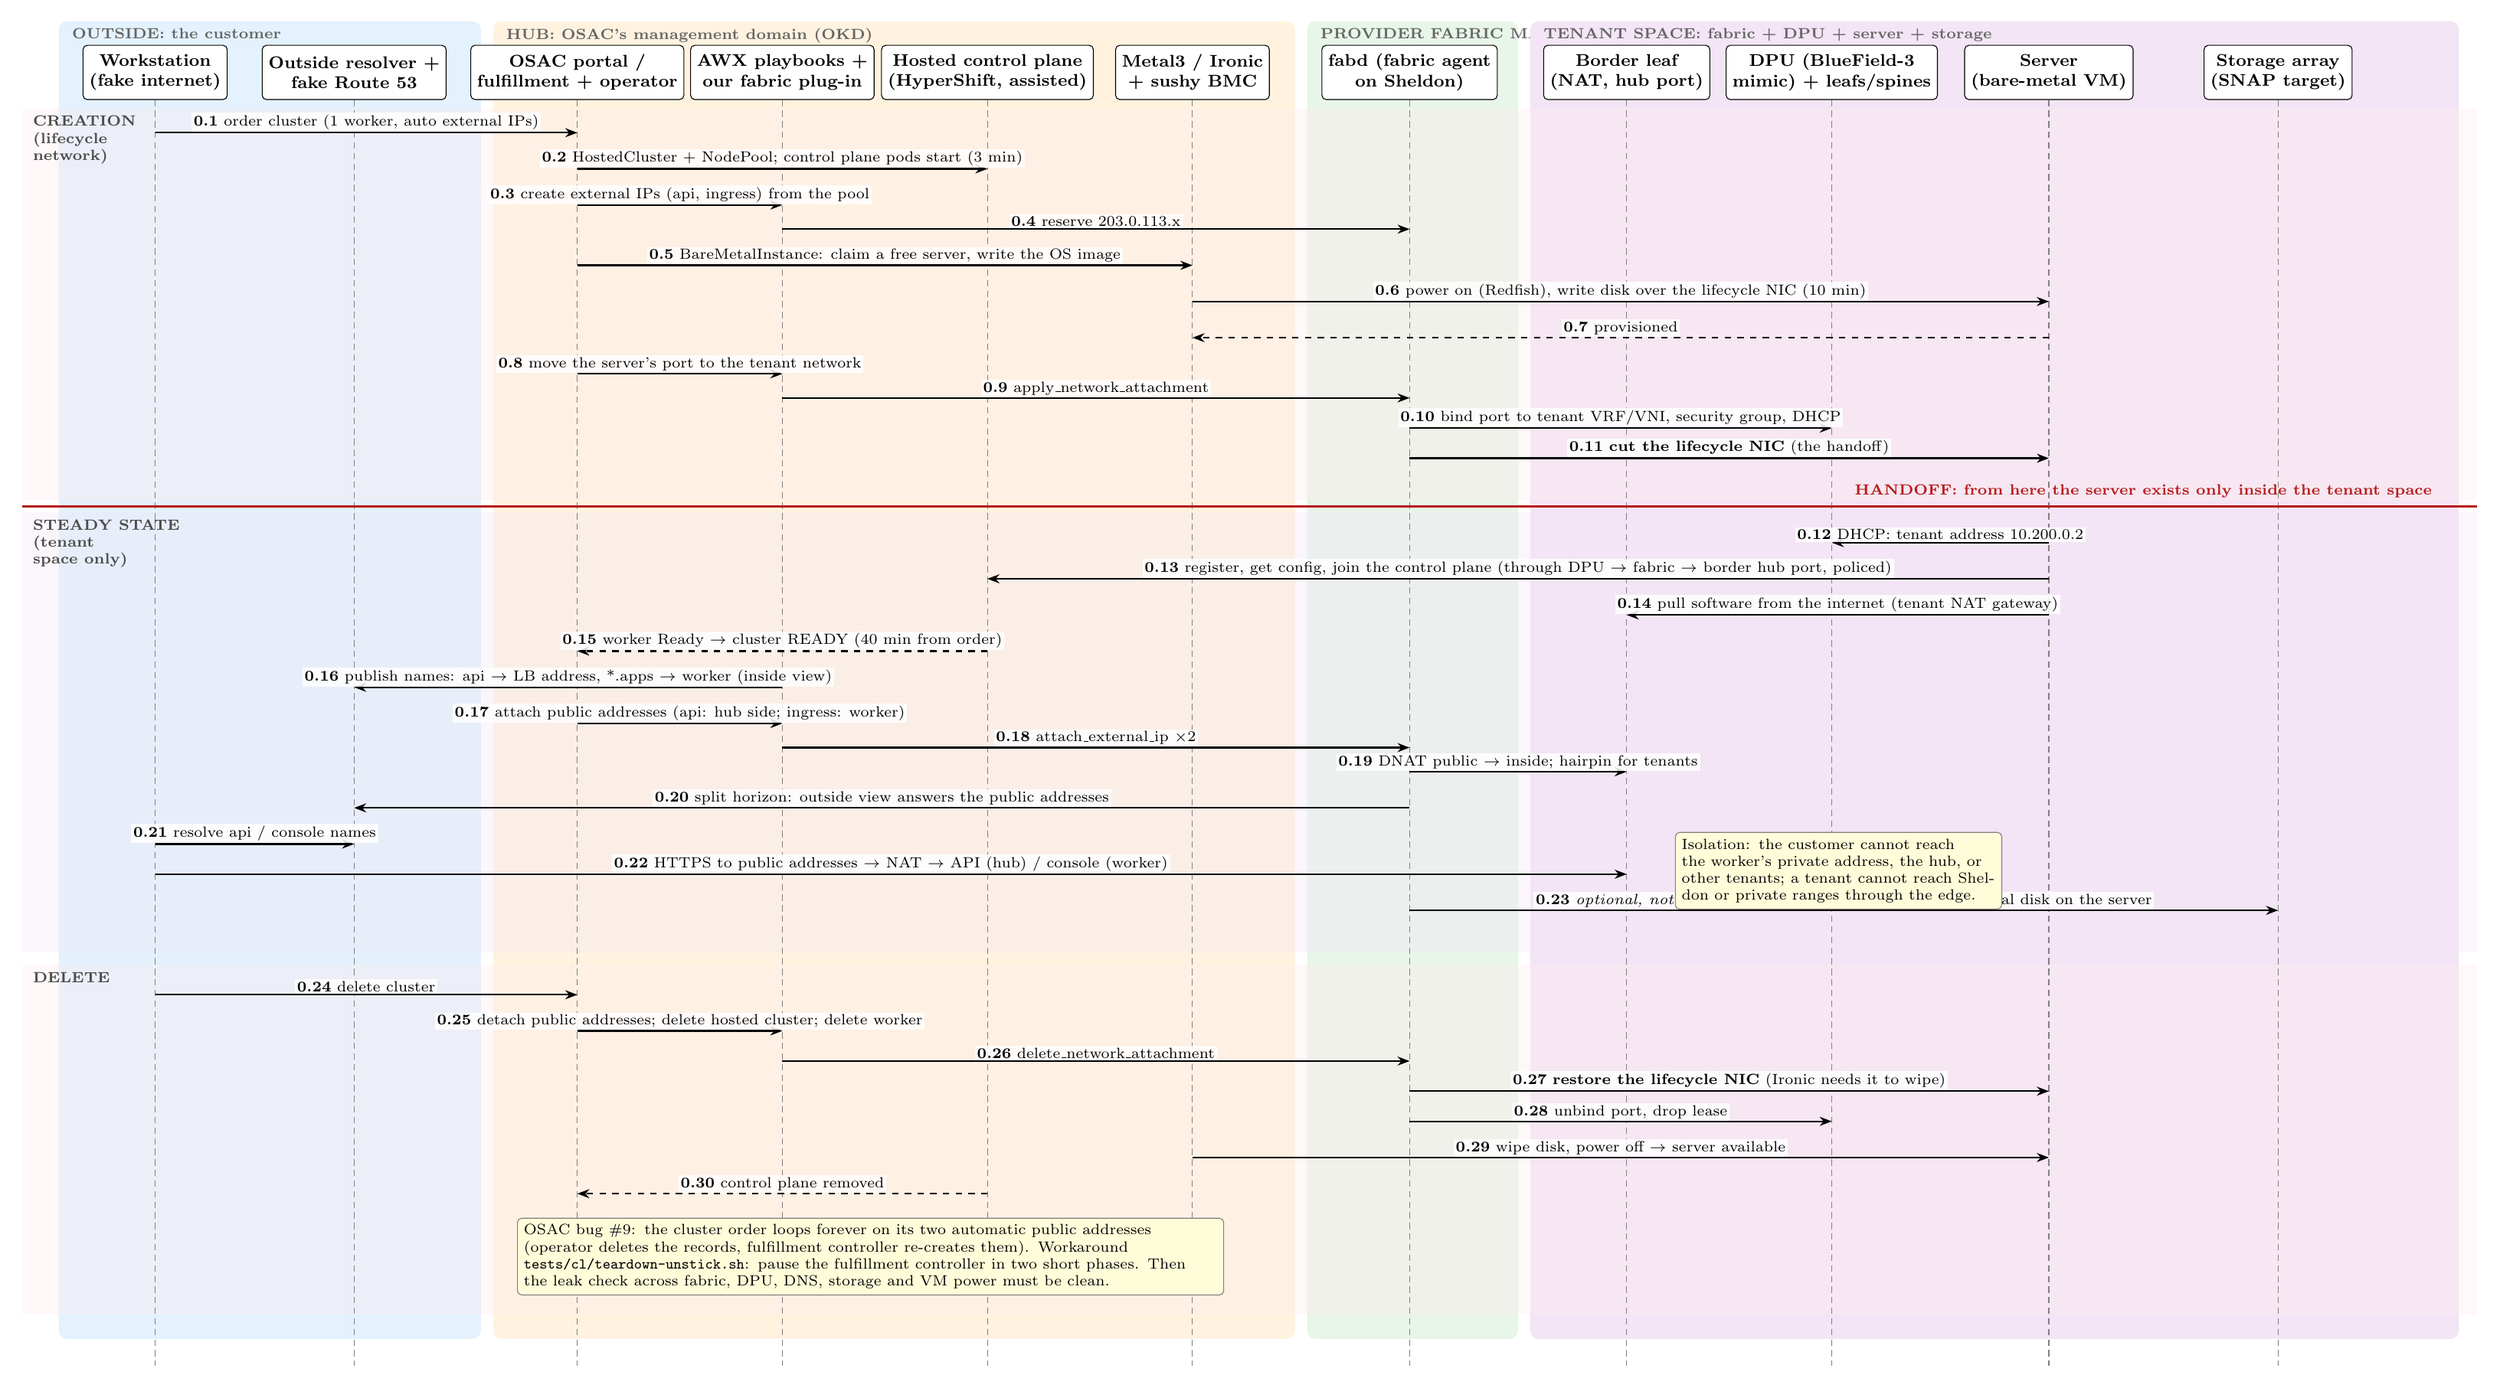
\begin{tikzpicture}[x=1cm,y=1cm]
\setlength{\sdH}{21cm}\setlength{\sdW}{39.5cm}
\bound{-0.6}{6.4}{OUTSIDE: the customer}{bOut}
\bound{6.6}{19.9}{HUB: OSAC's management domain (OKD)}{bHub}
\bound{20.1}{23.6}{PROVIDER FABRIC MANAGER}{bFab}
\bound{23.8}{39.2}{TENANT SPACE: fabric + DPU + server + storage}{bTen}
\lane{ws}{1.0}{Workstation\\(fake internet)}
\lane{dns}{4.3}{Outside resolver +\\fake Route 53}
\lane{osac}{8.0}{OSAC portal /\\fulfillment + operator}
\lane{awx}{11.4}{AWX playbooks +\\our fabric plug-in}
\lane{hcp}{14.8}{Hosted control plane\\(HyperShift, assisted)}
\lane{m3}{18.2}{Metal3 / Ironic\\+ sushy BMC}
\lane{fabd}{21.8}{fabd (fabric agent\\on Sheldon)}
\lane{bd}{25.4}{Border leaf\\(NAT, hub port)}
\lane{dpu}{28.8}{DPU (BlueField-3\\mimic) + leafs/spines}
\lane{srv}{32.4}{Server\\(bare-metal VM)}
\lane{arr}{36.2}{Storage array\\(SNAP target)}

\phase{0.6}{7.1}{CREATION\\(lifecycle\\network)}{bLife}
\phase{7.3}{14.6}{STEADY STATE\\(tenant\\space only)}{bTen}
\phase{14.8}{20.6}{DELETE}{bLife}

\msg{1.0}{ws}{osac}{order cluster (1 worker, auto external IPs)}
\msg{1.6}{osac}{hcp}{HostedCluster + NodePool; control plane pods start (3 min)}
\msg{2.2}{osac}{awx}{create external IPs (api, ingress) from the pool}
\msg{2.6}{awx}{fabd}{reserve 203.0.113.x}
\msg{3.2}{osac}{m3}{BareMetalInstance: claim a free server, write the OS image}
\msg{3.8}{m3}{srv}{power on (Redfish), write disk over the lifecycle NIC (10 min)}
\rmsg{4.4}{srv}{m3}{provisioned}
\msg{5.0}{osac}{awx}{move the server's port to the tenant network}
\msg{5.4}{awx}{fabd}{apply\_network\_attachment}
\msg{5.9}{fabd}{dpu}{bind port to tenant VRF/VNI, security group, DHCP}
\msg{6.4}{fabd}{srv}{\textbf{cut the lifecycle NIC} (the handoff)}
\draw[cHand,very thick] (-1.2,-7.2) -- (\sdW,-7.2) node[pos=.985,above left,font=\scriptsize\bfseries,text=cHand]{HANDOFF: from here the server exists only inside the tenant space};

\msg{7.8}{srv}{dpu}{DHCP: tenant address 10.200.0.2}
\msg{8.4}{srv}{hcp}{register, get config, join the control plane (through DPU $\to$ fabric $\to$ border hub port, policed)}
\msg{9.0}{srv}{bd}{pull software from the internet (tenant NAT gateway)}
\rmsg{9.6}{hcp}{osac}{worker Ready $\to$ cluster READY (40 min from order)}
\msg{10.2}{awx}{dns}{publish names: api $\to$ LB address, *.apps $\to$ worker (inside view)}
\msg{10.8}{osac}{awx}{attach public addresses (api: hub side; ingress: worker)}
\msg{11.2}{awx}{fabd}{attach\_external\_ip $\times$2}
\msg{11.6}{fabd}{bd}{DNAT public $\to$ inside; hairpin for tenants}
\msg{12.2}{fabd}{dns}{split horizon: outside view answers the public addresses}
\msg{12.8}{ws}{dns}{resolve api / console names}
\msg{13.3}{ws}{bd}{HTTPS to public addresses $\to$ NAT $\to$ API (hub) / console (worker)}
\msg{13.9}{fabd}{arr}{\textit{optional, not driven by OSAC yet:} SNAP volume $\to$ local disk on the server}
\note{12.6}{26.2}{5.2cm}{Isolation: the customer cannot reach the worker's private address, the hub, or other tenants; a tenant cannot reach Sheldon or private ranges through the edge.}

\msg{15.3}{ws}{osac}{delete cluster}
\msg{15.9}{osac}{awx}{detach public addresses; delete hosted cluster; delete worker}
\msg{16.4}{awx}{fabd}{delete\_network\_attachment}
\msg{16.9}{fabd}{srv}{\textbf{restore the lifecycle NIC} (Ironic needs it to wipe)}
\msg{17.4}{fabd}{dpu}{unbind port, drop lease}
\msg{18.0}{m3}{srv}{wipe disk, power off $\to$ server available}
\rmsg{18.6}{hcp}{osac}{control plane removed}
\note{19.0}{7.0}{11.5cm}{OSAC bug \#9: the cluster order loops forever on its two automatic public addresses (operator deletes the records, fulfillment controller re-creates them). Workaround \texttt{tests/cl/teardown-unstick.sh}: pause the fulfillment controller in two short phases. Then the leak check across fabric, DPU, DNS, storage and VM power must be clean.}
\end{tikzpicture}}

\newpage
% =============================================================================
\section*{2. Low level: provisioning the worker and the handoff from the lifecycle network to the tenant space}
\noindent\textit{What happens between ``OSAC claims a server'' and ``the server has a tenant address''. The red line is the moment the server stops being reachable on the lifecycle network and lives only behind its DPU.}\par\medskip
\stepcounter{sddiag}\setcounter{sdstep}{0}\resizebox{\textwidth}{!}{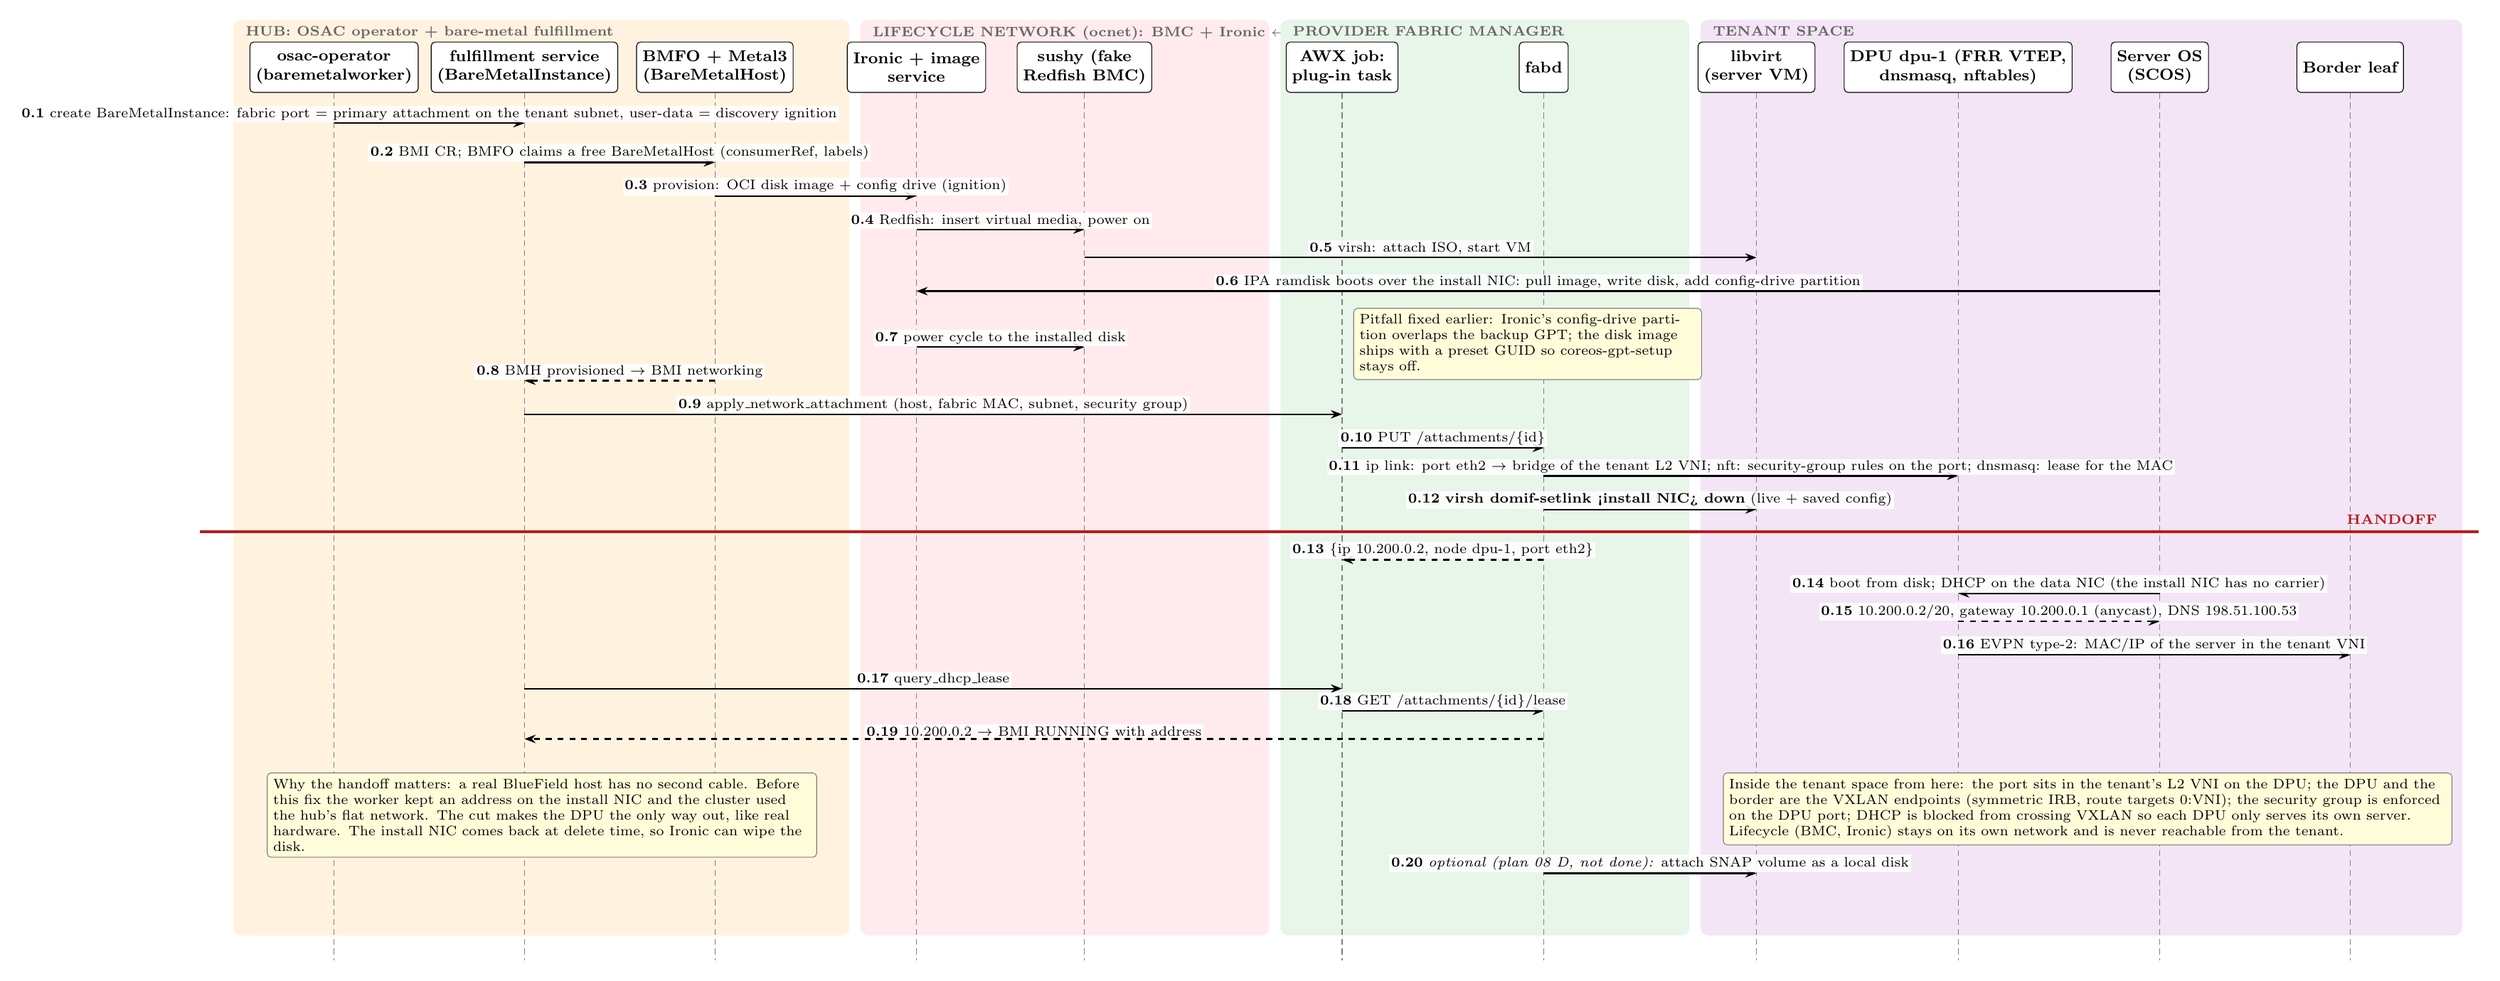
\begin{tikzpicture}[x=1cm,y=1cm]
\setlength{\sdH}{15.5cm}\setlength{\sdW}{39.5cm}
\bound{-0.6}{10.4}{HUB: OSAC operator + bare-metal fulfillment}{bHub}
\bound{10.6}{17.9}{LIFECYCLE NETWORK (ocnet): BMC + Ironic $\leftrightarrow$ server's install NIC}{bLife}
\bound{18.1}{25.4}{PROVIDER FABRIC MANAGER}{bFab}
\bound{25.6}{39.2}{TENANT SPACE}{bTen}
\lane{op}{1.2}{osac-operator\\(baremetalworker)}
\lane{ful}{4.6}{fulfillment service\\(BareMetalInstance)}
\lane{bmfo}{8.0}{BMFO + Metal3\\(BareMetalHost)}
\lane{ir}{11.6}{Ironic + image\\service}
\lane{bmc}{14.6}{sushy (fake\\Redfish BMC)}
\lane{awx}{19.2}{AWX job:\\plug-in task}
\lane{fabd}{22.8}{fabd}
\lane{lv}{26.6}{libvirt\\(server VM)}
\lane{dpu}{30.2}{DPU dpu-1 (FRR VTEP,\\dnsmasq, nftables)}
\lane{srv}{33.8}{Server OS\\(SCOS)}
\lane{bd}{37.2}{Border leaf}

\msg{1.0}{op}{ful}{create BareMetalInstance: fabric port = primary attachment on the tenant subnet, user-data = discovery ignition}
\msg{1.7}{ful}{bmfo}{BMI CR; BMFO claims a free BareMetalHost (consumerRef, labels)}
\msg{2.3}{bmfo}{ir}{provision: OCI disk image + config drive (ignition)}
\msg{2.9}{ir}{bmc}{Redfish: insert virtual media, power on}
\msg{3.4}{bmc}{lv}{virsh: attach ISO, start VM}
\msg{4.0}{srv}{ir}{IPA ramdisk boots over the install NIC: pull image, write disk, add config-drive partition}
\note{4.3}{19.4}{6.0cm}{Pitfall fixed earlier: Ironic's config-drive partition overlaps the backup GPT; the disk image ships with a preset GUID so coreos-gpt-setup stays off.}
\msg{5.0}{ir}{bmc}{power cycle to the installed disk}
\rmsg{5.6}{bmfo}{ful}{BMH provisioned $\to$ BMI networking}
\msg{6.2}{ful}{awx}{apply\_network\_attachment (host, fabric MAC, subnet, security group)}
\msg{6.8}{awx}{fabd}{PUT /attachments/\{id\}}
\msg{7.3}{fabd}{dpu}{ip link: port eth2 $\to$ bridge of the tenant L2 VNI; nft: security-group rules on the port; dnsmasq: lease for the MAC}
\msg{7.9}{fabd}{lv}{\textbf{virsh domif-setlink <install NIC> down} (live + saved config)}
\draw[cHand,very thick] (-1.2,-8.3) -- (\sdW,-8.3) node[pos=.985,above left,font=\scriptsize\bfseries,text=cHand]{HANDOFF};
\rmsg{8.8}{fabd}{awx}{\{ip 10.200.0.2, node dpu-1, port eth2\}}
\msg{9.4}{srv}{dpu}{boot from disk; DHCP on the data NIC (the install NIC has no carrier)}
\rmsg{9.9}{dpu}{srv}{10.200.0.2/20, gateway 10.200.0.1 (anycast), DNS 198.51.100.53}
\msg{10.5}{dpu}{bd}{EVPN type-2: MAC/IP of the server in the tenant VNI}
\msg{11.1}{ful}{awx}{query\_dhcp\_lease}
\msg{11.5}{awx}{fabd}{GET /attachments/\{id\}/lease}
\rmsg{12.0}{fabd}{ful}{10.200.0.2 $\to$ BMI RUNNING with address}
\note{12.6}{0.0}{9.6cm}{Why the handoff matters: a real BlueField host has no second cable. Before this fix the worker kept an address on the install NIC and the cluster used the hub's flat network. The cut makes the DPU the only way out, like real hardware. The install NIC comes back at delete time, so Ironic can wipe the disk.}
\note{12.6}{26.0}{12.8cm}{Inside the tenant space from here: the port sits in the tenant's L2 VNI on the DPU; the DPU and the border are the VXLAN endpoints (symmetric IRB, route targets 0:VNI); the security group is enforced on the DPU port; DHCP is blocked from crossing VXLAN so each DPU only serves its own server. Lifecycle (BMC, Ironic) stays on its own network and is never reachable from the tenant.}
\msg{14.4}{fabd}{lv}{\textit{optional (plan 08 D, not done):} attach SNAP volume as a local disk}
\end{tikzpicture}}

\newpage
% =============================================================================
\section*{3. Low level: the worker joins the control plane across the hub boundary}
\noindent\textit{The worker is inside the tenant space and must reach three services on the hub. The hub is attached to the border leaf as a shared service; each tenant VRF gets a narrow, policed route to it, and everything leaving the hub port is disguised as the border, so the hub needs no route back into tenants.}\par\medskip
\stepcounter{sddiag}\setcounter{sdstep}{0}\resizebox{\textwidth}{!}{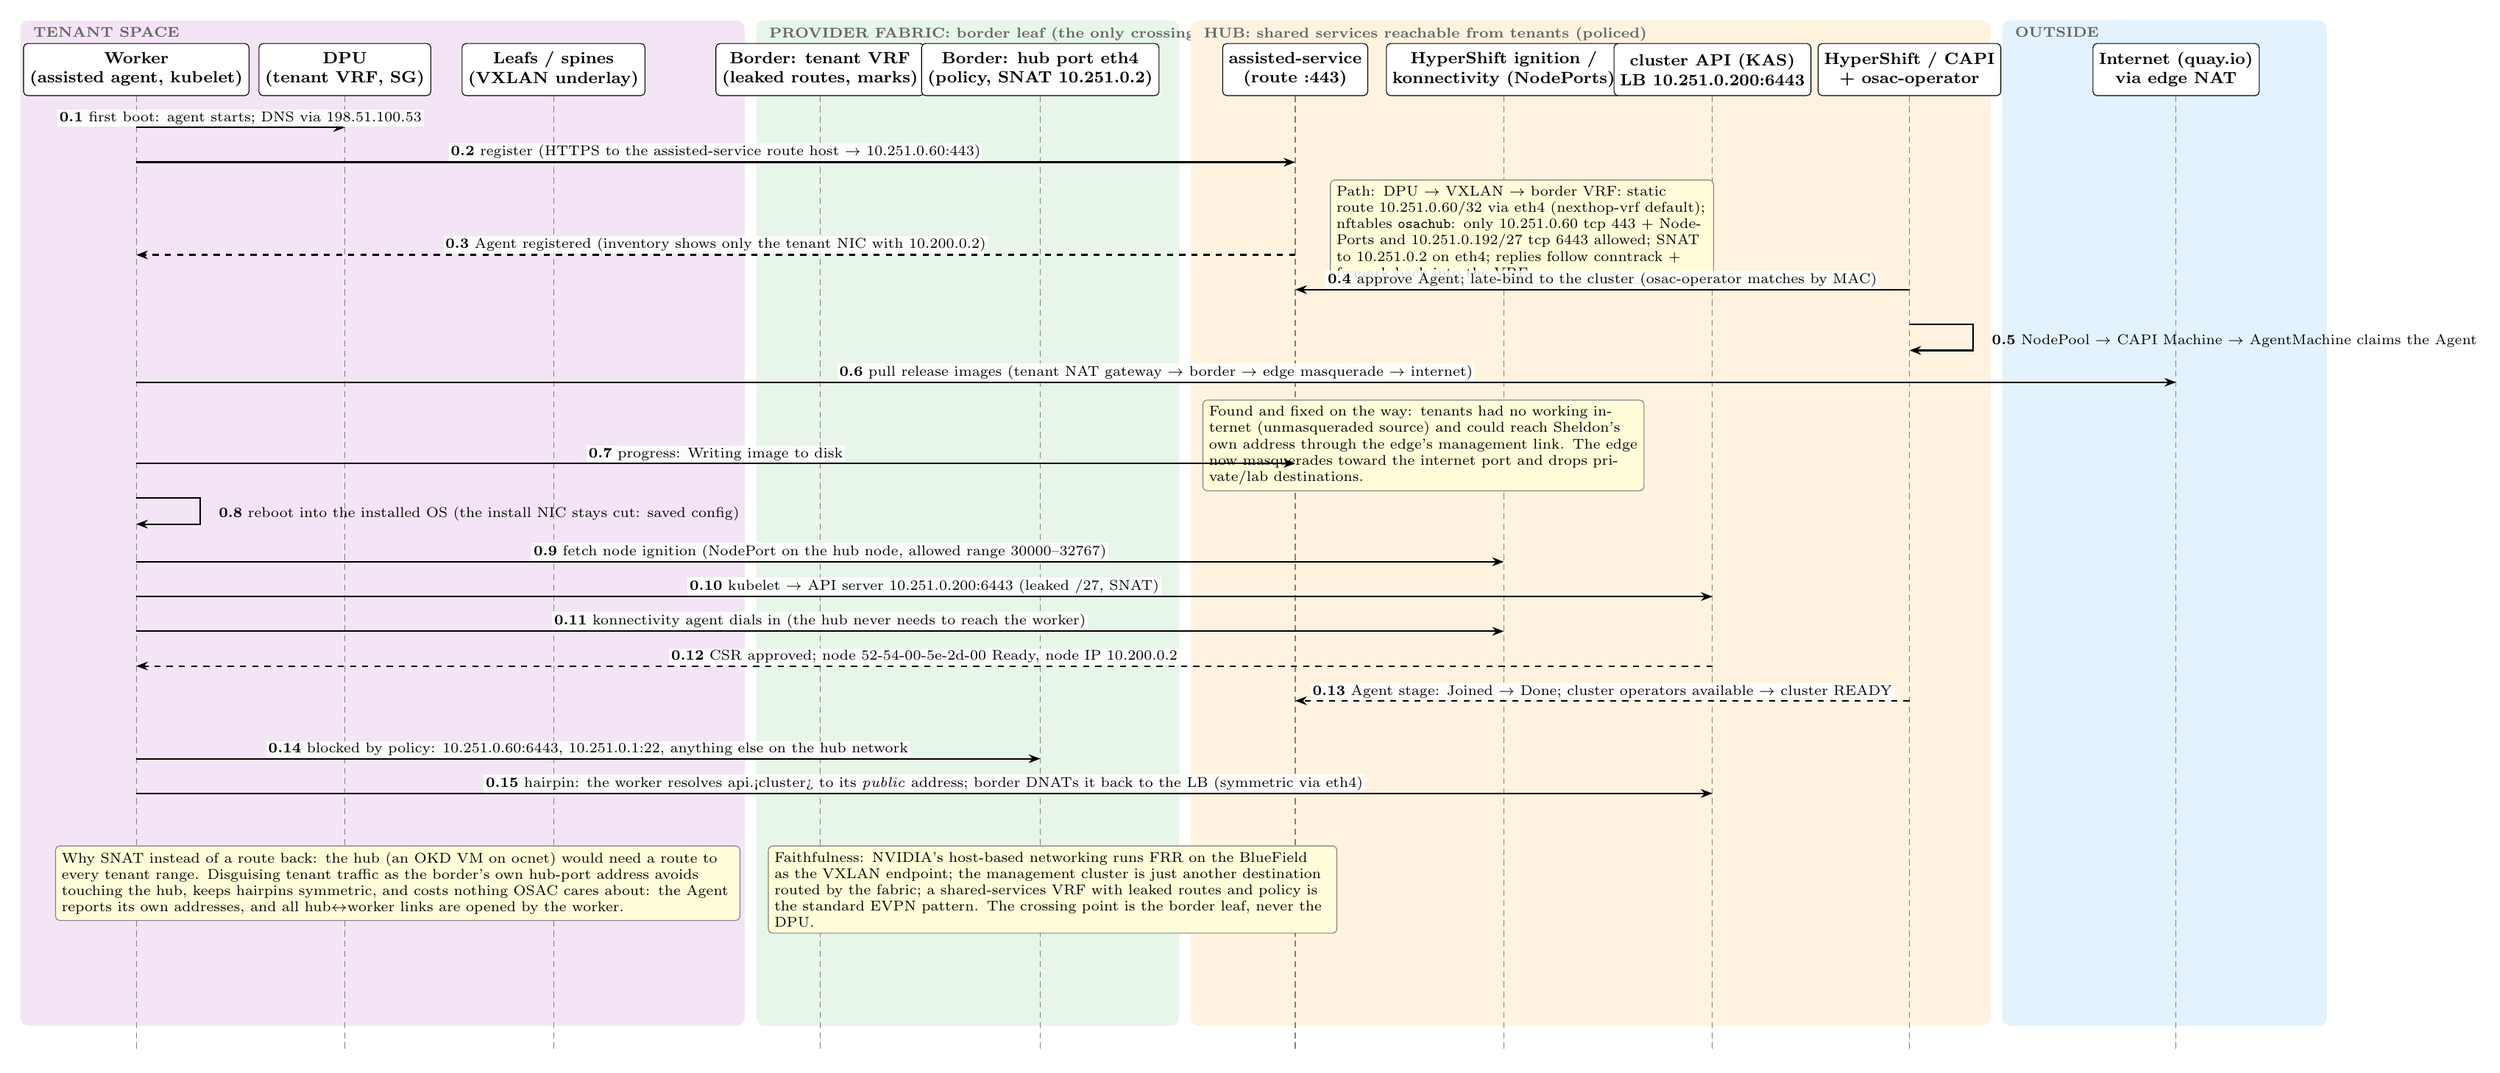
\begin{tikzpicture}[x=1cm,y=1cm]
\setlength{\sdH}{16.5cm}\setlength{\sdW}{39.5cm}
\bound{-0.6}{11.9}{TENANT SPACE}{bTen}
\bound{12.1}{19.4}{PROVIDER FABRIC: border leaf (the only crossing point)}{bFab}
\bound{19.6}{33.4}{HUB: shared services reachable from tenants (policed)}{bHub}
\bound{33.6}{39.2}{OUTSIDE}{bOut}
\lane{srv}{1.4}{Worker\\(assisted agent, kubelet)}
\lane{dpu}{5.0}{DPU\\(tenant VRF, SG)}
\lane{fab}{8.6}{Leafs / spines\\(VXLAN underlay)}
\lane{vrf}{13.2}{Border: tenant VRF\\(leaked routes, marks)}
\lane{hp}{17.0}{Border: hub port eth4\\(policy, SNAT 10.251.0.2)}
\lane{as}{21.4}{assisted-service\\(route :443)}
\lane{ign}{25.0}{HyperShift ignition /\\konnectivity (NodePorts)}
\lane{kas}{28.6}{cluster API (KAS)\\LB 10.251.0.200:6443}
\lane{hs}{32.0}{HyperShift / CAPI\\+ osac-operator}
\lane{inet}{36.6}{Internet (quay.io)\\via edge NAT}

\msg{1.0}{srv}{dpu}{first boot: agent starts; DNS via 198.51.100.53}
\msg{1.6}{srv}{as}{register (HTTPS to the assisted-service route host $\to$ 10.251.0.60:443)}
\note{1.9}{22.0}{6.4cm}{Path: DPU $\to$ VXLAN $\to$ border VRF: static route 10.251.0.60/32 via eth4 (nexthop-vrf default); nftables \texttt{osachub}: only 10.251.0.60 tcp 443 + NodePorts and 10.251.0.192/27 tcp 6443 allowed; SNAT to 10.251.0.2 on eth4; replies follow conntrack + fwmark back into the VRF.}
\rmsg{3.2}{as}{srv}{Agent registered (inventory shows only the tenant NIC with 10.200.0.2)}
\msg{3.8}{hs}{as}{approve Agent; late-bind to the cluster (osac-operator matches by MAC)}
\self{4.4}{hs}{NodePool $\to$ CAPI Machine $\to$ AgentMachine claims the Agent}
\msg{5.4}{srv}{inet}{pull release images (tenant NAT gateway $\to$ border $\to$ edge masquerade $\to$ internet)}
\note{5.7}{19.8}{7.4cm}{Found and fixed on the way: tenants had no working internet (unmasqueraded source) and could reach Sheldon's own address through the edge's management link. The edge now masquerades toward the internet port and drops private/lab destinations.}
\msg{6.8}{srv}{as}{progress: Writing image to disk}
\self{7.4}{srv}{reboot into the installed OS (the install NIC stays cut: saved config)}
\msg{8.5}{srv}{ign}{fetch node ignition (NodePort on the hub node, allowed range 30000--32767)}
\msg{9.1}{srv}{kas}{kubelet $\to$ API server 10.251.0.200:6443 (leaked /27, SNAT)}
\msg{9.7}{srv}{ign}{konnectivity agent dials in (the hub never needs to reach the worker)}
\rmsg{10.3}{kas}{srv}{CSR approved; node 52-54-00-5e-2d-00 Ready, node IP 10.200.0.2}
\rmsg{10.9}{hs}{as}{Agent stage: Joined $\to$ Done; cluster operators available $\to$ cluster READY}
\msg{11.9}{srv}{hp}{blocked by policy: 10.251.0.60:6443, 10.251.0.1:22, anything else on the hub network}
\msg{12.5}{srv}{kas}{hairpin: the worker resolves api.<cluster> to its \textit{public} address; border DNATs it back to the LB (symmetric via eth4)}
\note{13.4}{0.0}{11.6cm}{Why SNAT instead of a route back: the hub (an OKD VM on ocnet) would need a route to every tenant range. Disguising tenant traffic as the border's own hub-port address avoids touching the hub, keeps hairpins symmetric, and costs nothing OSAC cares about: the Agent reports its own addresses, and all hub$\leftrightarrow$worker links are opened by the worker.}
\note{13.4}{12.3}{9.6cm}{Faithfulness: NVIDIA's host-based networking runs FRR on the BlueField as the VXLAN endpoint; the management cluster is just another destination routed by the fabric; a shared-services VRF with leaked routes and policy is the standard EVPN pattern. The crossing point is the border leaf, never the DPU.}
\end{tikzpicture}}

\newpage
% =============================================================================
\section*{4. Low level: publishing the cluster and reaching it from outside}
\noindent\textit{How a customer on the fake internet reaches a cluster that lives inside a tenant. OSAC publishes inside addresses and allocates public ones; our fabric manager does the NAT at the border and the split-horizon DNS. Two OSAC bugs sit in this flow.}\par\medskip
\stepcounter{sddiag}\setcounter{sdstep}{0}\resizebox{\textwidth}{!}{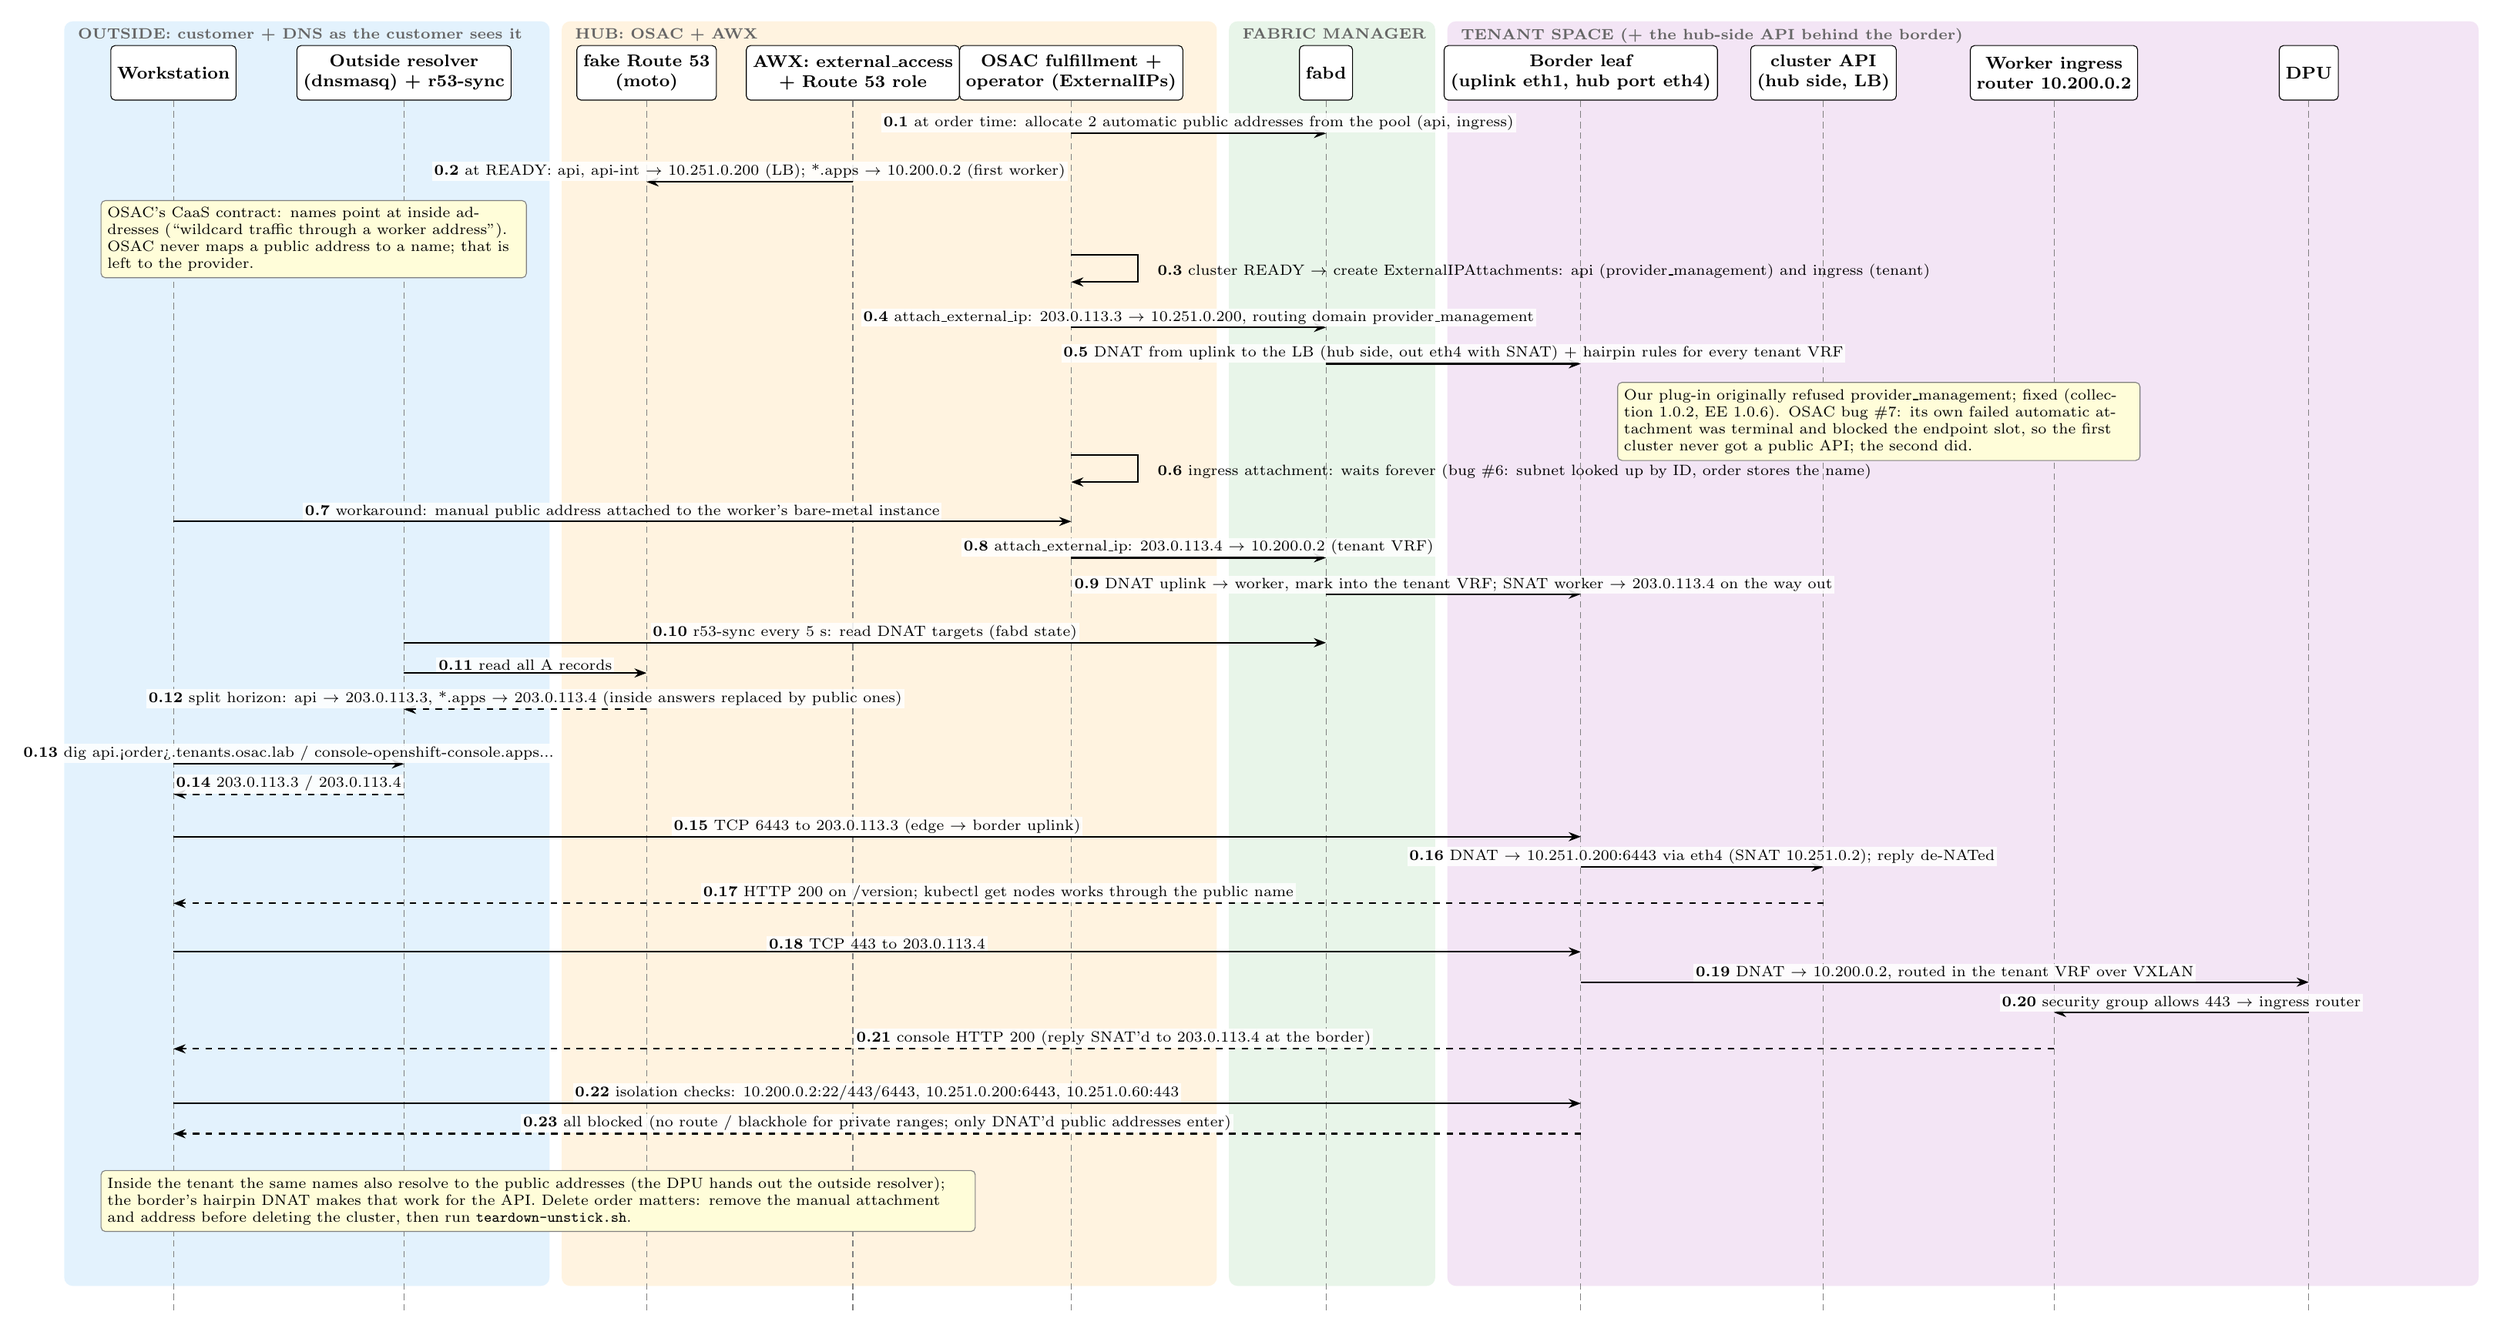
\begin{tikzpicture}[x=1cm,y=1cm]
\setlength{\sdH}{20cm}\setlength{\sdW}{39.5cm}
\bound{-0.6}{7.4}{OUTSIDE: customer + DNS as the customer sees it}{bOut}
\bound{7.6}{18.4}{HUB: OSAC + AWX}{bHub}
\bound{18.6}{22.0}{FABRIC MANAGER}{bFab}
\bound{22.2}{39.2}{TENANT SPACE (+ the hub-side API behind the border)}{bTen}
\lane{ws}{1.2}{Workstation}
\lane{res}{5.0}{Outside resolver\\(dnsmasq) + r53-sync}
\lane{r53}{9.0}{fake Route 53\\(moto)}
\lane{ea}{12.4}{AWX: external\_access\\+ Route 53 role}
\lane{op}{16.0}{OSAC fulfillment +\\operator (ExternalIPs)}
\lane{fabd}{20.2}{fabd}
\lane{bd}{24.4}{Border leaf\\(uplink eth1, hub port eth4)}
\lane{kas}{28.4}{cluster API\\(hub side, LB)}
\lane{wk}{32.2}{Worker ingress\\router 10.200.0.2}
\lane{dpu}{36.4}{DPU}

\msg{1.0}{op}{fabd}{at order time: allocate 2 automatic public addresses from the pool (api, ingress)}
\msg{1.8}{ea}{r53}{at READY: api, api-int $\to$ 10.251.0.200 (LB); *.apps $\to$ 10.200.0.2 (first worker)}
\note{2.1}{0.0}{6.8cm}{OSAC's CaaS contract: names point at inside addresses (``wildcard traffic through a worker address''). OSAC never maps a public address to a name; that is left to the provider.}
\self{3.0}{op}{cluster READY $\to$ create ExternalIPAttachments: api (provider\_management) and ingress (tenant)}
\msg{4.2}{op}{fabd}{attach\_external\_ip: 203.0.113.3 $\to$ 10.251.0.200, routing domain provider\_management}
\msg{4.8}{fabd}{bd}{DNAT from uplink to the LB (hub side, out eth4 with SNAT) + hairpin rules for every tenant VRF}
\note{5.1}{25.0}{8.4cm}{Our plug-in originally refused provider\_management; fixed (collection 1.0.2, EE 1.0.6). OSAC bug \#7: its own failed automatic attachment was terminal and blocked the endpoint slot, so the first cluster never got a public API; the second did.}
\self{6.3}{op}{ingress attachment: waits forever (bug \#6: subnet looked up by ID, order stores the name)}
\msg{7.4}{ws}{op}{workaround: manual public address attached to the worker's bare-metal instance}
\msg{8.0}{op}{fabd}{attach\_external\_ip: 203.0.113.4 $\to$ 10.200.0.2 (tenant VRF)}
\msg{8.6}{fabd}{bd}{DNAT uplink $\to$ worker, mark into the tenant VRF; SNAT worker $\to$ 203.0.113.4 on the way out}
\msg{9.4}{res}{fabd}{r53-sync every 5 s: read DNAT targets (fabd state)}
\msg{9.9}{res}{r53}{read all A records}
\rmsg{10.5}{r53}{res}{split horizon: api $\to$ 203.0.113.3, *.apps $\to$ 203.0.113.4 (inside answers replaced by public ones)}
\msg{11.4}{ws}{res}{dig api.<order>.tenants.osac.lab / console-openshift-console.apps...}
\rmsg{11.9}{res}{ws}{203.0.113.3 / 203.0.113.4}
\msg{12.6}{ws}{bd}{TCP 6443 to 203.0.113.3 (edge $\to$ border uplink)}
\msg{13.1}{bd}{kas}{DNAT $\to$ 10.251.0.200:6443 via eth4 (SNAT 10.251.0.2); reply de-NATed}
\rmsg{13.7}{kas}{ws}{HTTP 200 on /version; kubectl get nodes works through the public name}
\msg{14.5}{ws}{bd}{TCP 443 to 203.0.113.4}
\msg{15.0}{bd}{dpu}{DNAT $\to$ 10.200.0.2, routed in the tenant VRF over VXLAN}
\msg{15.5}{dpu}{wk}{security group allows 443 $\to$ ingress router}
\rmsg{16.1}{wk}{ws}{console HTTP 200 (reply SNAT'd to 203.0.113.4 at the border)}
\msg{17.0}{ws}{bd}{isolation checks: 10.200.0.2:22/443/6443, 10.251.0.200:6443, 10.251.0.60:443}
\rmsg{17.5}{bd}{ws}{all blocked (no route / blackhole for private ranges; only DNAT'd public addresses enter)}
\note{18.1}{0.0}{14.2cm}{Inside the tenant the same names also resolve to the public addresses (the DPU hands out the outside resolver); the border's hairpin DNAT makes that work for the API. Delete order matters: remove the manual attachment and address before deleting the cluster, then run \texttt{teardown-unstick.sh}.}
\end{tikzpicture}}
\end{document}
